\chapter{Implémentations et synthèse de texture}
\label{ch:chapitre2}

Le travail décrit dans ce manuscrit est une étude exploratoire du modèle local multirésolution. En particulier le rôle de la congruence de phases appliquée dans le contexte de la synthèse de texture est examiné. La mise en application des concepts exposés précédemment ainsi que les résultats obtenus sont le sujet de la partie qui suit.

\section{Implémentation}

Les concepts d'énergie locale et de signal monogène sont des notions peu communes dans le traitement d'image, aucune librairie standard ne les implémente à notre connaissance. L'implémentation des algorithmes pour mettre en place le modèle local multirésolution est une des réalisations de ce travail. Le choix du logiciel pour faire ces implémentations a été une question importante.


\paragraph{OpenCV}

Malgré l'objectif final de travailler sur de la synthèse de texture, la première réalisation a été le développement d'un petit logiciel pour pouvoir itérer rapidement et expérimenter avec les concepts de base du modèle local multirésolution sur des images, sans prendre en compte les problématiques de la synthèse. Pour cela, un logiciel utilisant \cpp avec la librairie OpenCV~\cite{opencv_library} a été mis au point. OpenCV est une librairie standard de traitement d'image en temps réel et de vision par ordinateur, disponible pour les langages de programmation \cpp, Python et Java. Les images y sont représentées comme des matrices et les opérations de bas niveau courantes du traitement d'image y sont implémentées, comme la lecture, l'écriture, l'affichage, le filtrage, la convolution et autres. Le logiciel élaboré permet à un utilisateur de créer, visualiser et modifier les pyramides d'une image d'entrée, ainsi que de calculer et visualiser la congruence de phases. Avec ces fonctionnalités, des expérimentations ont été faites pour voir l'effet de différentes modifications et reconstructions de la pyramide de Riesz d'une image.

\bigskip

Plusieurs raisons ont ensuite motivé le choix de changer d'implémentation. Après avoir expérimenté avec la congruence de phases sur des images, la prochaine étape était de travailler avec des textures, c'est-à-dire faire de la synthèse dans le cadre du pipeline graphique traditionnel. L'objectif était de synthétiser une texture à projeter sur une surface, potentiellement infinie, dans le but de la recouvrir. Dans un tel contexte, plusieurs problématiques surviennent. Pour être mise en place dans le pipeline graphique, la synthèse de texture doit pouvoir se faire dans le \textit{fragment shader}. Pour être exécutée dans le \textit{fragment shader}, une méthode de reconstruction parallélisable doit être utilisée pour profiter de la carte graphique. La méthode utilisée jusque-là ne pouvait pas être parallélisée à cause des convolutions impliquées dans le processus. Des questions de projection et de filtrage jusque-là non existantes furent nécessaires à considérer pour la synthèse de texture.

\bigskip

Parallèlement, notre laboratoire de recherche a accueilli de nouveaux membres travaillant sur la synthèse de texture. La mise en place d'un logiciel servant de base de travail commune pour les personnes faisant de la synthèse de texture est devenue une préoccupation. Pour mettre au point un logiciel commun, plusieurs options ont été considérées. Les options majeures étaient le développement d'un moteur de rendu personnalisé et adapté aux besoins de la synthèse ou l'utilisation d'un moteur de jeu existant, Unity3D~\cite{unity_engine} ou Unreal Engine~\cite{unreal_engine}. Le problème d'un moteur personnalisé est qu'il implique une ré-implémentation de plusieurs fonctionnalités courantes, donc beaucoup de redondance dans le travail. Unity3D et Unreal Engine, eux, malgré leur renommée et vaste utilisation dans l'industrie, avaient le désavantage de ne pas offrir la flexibilité de manipuler les textures nécessaire. L'option retenue est une autre alternative, le moteur de jeu Godot~\cite{godot_game_engine}.

\paragraph{Godot}

Godot est un logiciel libre et gratuit, moteur de jeu 2D et 3D, qui permet de faire du rendu temps-réel. L'utilisation de Godot permet de s'intéresser aux problématiques de la synthèse de texture, ce que ne permettait pas OpenCV. Bien que moins populaire que Unity et Unreal Engine, Godot est une solution qui croit en notoriété, surtout dans la recherche en informatique graphique. Les principaux avantages de Godot, et la raison de sa montée en popularité, et sa légèreté et sa flexibilité. Godot permet facilement d'écrire des modules personnalisés ou de modifier du code source pour s'adapter aux besoins des utilisateurs. C'est ce que nous avons fait avec Nicolas Lutz, postdoctorant du laboratoire. Un travail conjoint a été réalisé pour développer \textit{TexSyn}, une librairie \cpp de traitement d'image et de synthèse de texture pour Godot.

\bigskip

Godot a une classe qui gère les textures, mais la manipuler est compliqué et peu efficace pour des opérations d'accès direct nécessaires à la synthèse. La librairie \textit{TexSyn} définit une classe d'image plus pratique à utiliser, avec toutes les opérations requises. La classe d'image de \textit{TexSyn} est ensuite interfacée avec la classe d'image de Godot pour être utilisable depuis les scripts Godot. Dans ce cadre de travail, les pyramides d'images sont construites en pré-calcul sur l'unité centrale de traitement. Les pyramides sont stockées dans des atlas de textures, puis chargées en mémoire sur la carte graphique. La reconstruction est faite depuis les \textit{shaders}, en temps réel, en utilisant les pyramides stockées dans les atlas. La reconstruction est cependant soumise à des problèmes de filtrage (voir figure~\ref{fig:texsyn-reconstruction}), car la convolution par filtre utilisée pour faire le lissage ne peut pas être appliquée depuis le \textit{fragment shader} pour des raisons d'accès parallèle. La librairie \textit{TexSyn} est ensuite utilisée pour développer une méthode de syntèse pouvant traiter des textures à structure irrégulière. La méthode de synthèse proposée est basée sur un échantillonneur préservant la congruence de phases, détaillé plus loin dans ce chapitre.

\begin{figure}
    \centering
    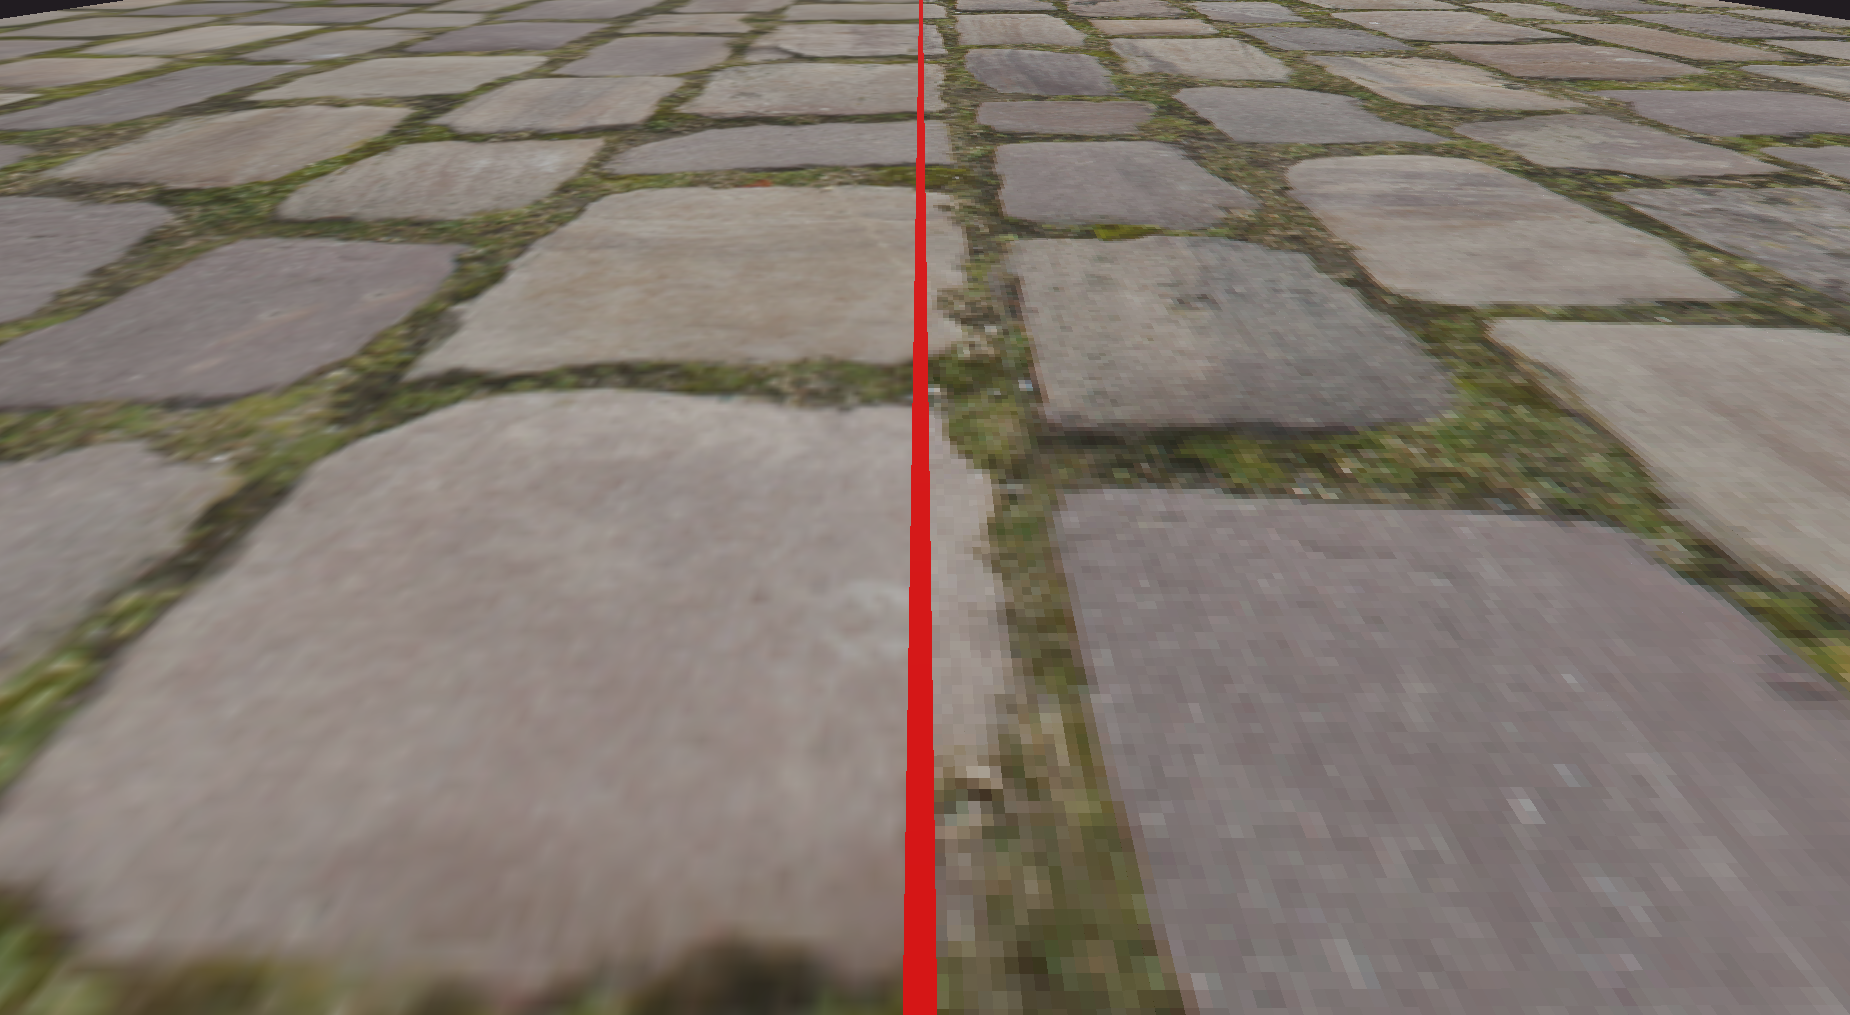
\includegraphics[width=0.9\textwidth]{contenu/resources/images/reconstruction_cpu_vs_gpu}
    \caption[Reconstruction de texture dans \textit{TexSyn}]{Reconstruction de la pyramide de Riesz d'une texture, hors-ligne depuis l'unité centrale de traitement (gauche) et en temps-réel depuis le \textit{fragment shader} (droite). Des artefacts de filtrage sont visibles sur la reconstruction en temps-réel.}
    \label{fig:texsyn-reconstruction}
\end{figure}


\section{Sélection de niveaux de fréquences}

La mise au point de la congruence de phases et l'utilisation d'un contexte multirésolution permettent de visualiser explicitement que les différents niveaux de structure trouvés dans une image sont liés à différents niveaux de d'échelle. Nous avons émis l'hypothèse que chaque niveau de structure distingué dans une image s'exprime comme la congruence en phases d'un sous-ensemble fréquentiel. Autrement dit, chaque échelle de structure est créée par un sous-ensemble de niveaux de la pyramide d'image. Pour vérifier l'hypothèse, la sélection de sous-ensembles de niveaux de la pyramide lors du calcul de la congruence de phases a été étudiée avec
\begin{equation}
    PC_{\mathcal{S}}(\mathbf{x}) = \frac{W(x)E(\mathbf{x})}{\epsilon + \sum_{n\in\mathcal{S}} A_{n}(\mathbf{x})},
\end{equation}
où $\mathcal{S}$ est un sous-ensemble de niveaux de la pyramide. L'algorithme a été testé avec tous les $\mathcal{S} = \llbracket a, b\rrbracket$ où $1 \leq a \leq b \leq d$. La sélection de niveaux a permis de confirmer que différents niveaux de structure sont bien causés par différents sous-ensembles fréquentiels, comme montré à la figure~\ref{fig:pc-selection-niveaux}.

\bigskip

\begin{figure}
    \centering
    \begin{subfigure}[b]{.25\textwidth}
        \centering
        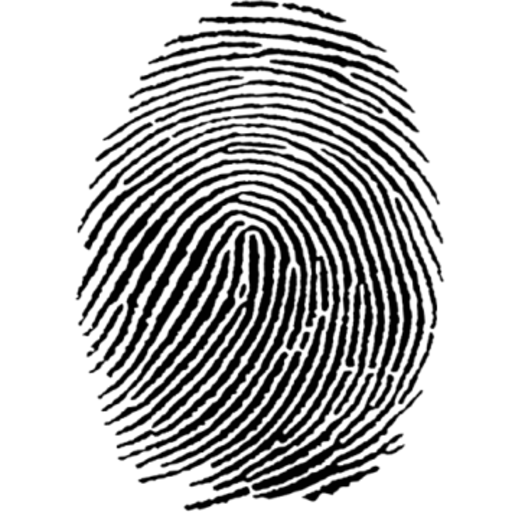
\includegraphics[width=\textwidth]{contenu/resources/images/fingerprint}
        \caption{Image originale}
    \end{subfigure}
    \hfill
    \begin{subfigure}[b]{.25\textwidth}
        \centering
        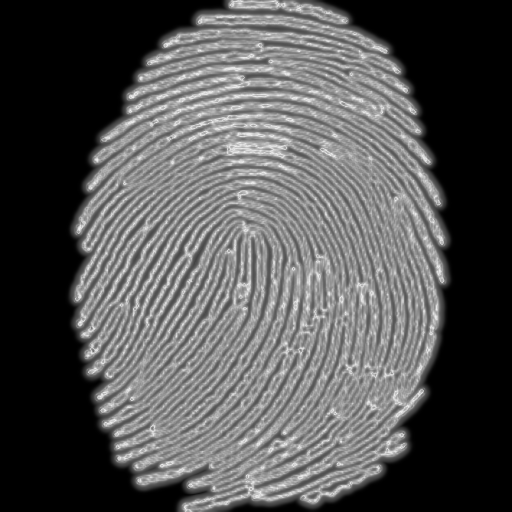
\includegraphics[width=\textwidth]{contenu/resources/images/pc_layer_0_1}
        \caption{Niveaux 0 et 1}
    \end{subfigure}
    \hfill
    \begin{subfigure}[b]{.25\textwidth}
        \centering
        
\includegraphics[width=\textwidth]{contenu/resources/images/pc_layer_2_depth-1}
        \caption{Niveaux 2 à $d-1$}
    \end{subfigure}

    \caption[Congruence de phases sur différents niveaux d'échelle]{Congruence de phases sur différents niveaux d'échelle. Sur les premiers niveaux (milieu), qui correspondent aux hautes fréquences, les détails fins ressortent. À l'inverse sur les derniers niveaux (droite), qui correspondent aux plus basses fréquences, c'est la structure globale, le contour de l'empreinte, qui apparait.}
    \label{fig:pc-selection-niveaux}
\end{figure}

Suite à cette observation, une méthode de sélection de niveaux de fréquences a été mise en place pour supprimer certains niveaux de la pyramide et observer l'effet sur la reconstruction. L'objectif était de pouvoir cibler certains niveaux de structure et les extraire de l'image. Cette méthode de sélection de niveaux a été mise application pour faire du filtrage de bandes de basses fréquences sur des textures de matériaux divers (voir figure~\ref{fig:filter-low-freq}) et gommer des tâches présentes sur les images.

\begin{figure}
    \centering
    \begin{subfigure}[b]{.25\textwidth}
        \centering
        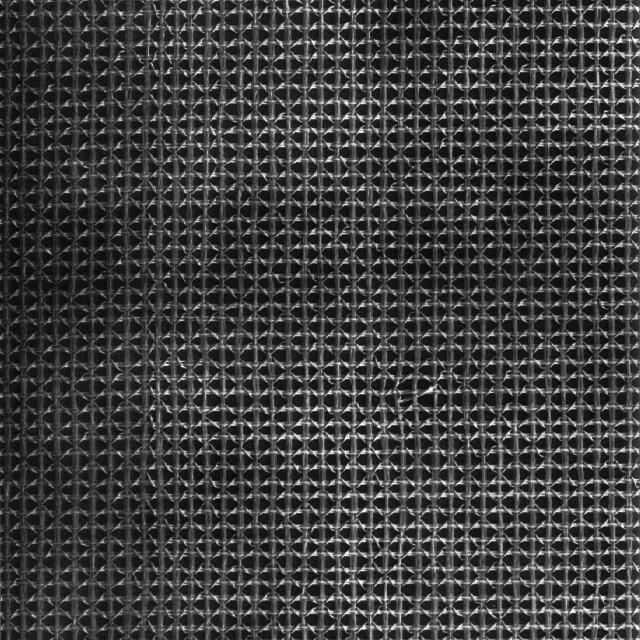
\includegraphics[width=\textwidth]{contenu/resources/images/lattice}
    \end{subfigure}
    \hspace{1em}
    \begin{subfigure}[b]{.25\textwidth}
        \centering
        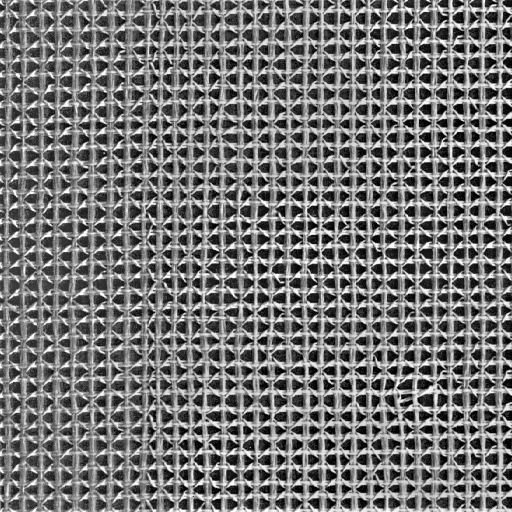
\includegraphics[width=\textwidth]{contenu/resources/images/lattice_filtered}
    \end{subfigure}
    \\
    \vspace{1em}
    \begin{subfigure}[b]{.25\textwidth}
        \centering
        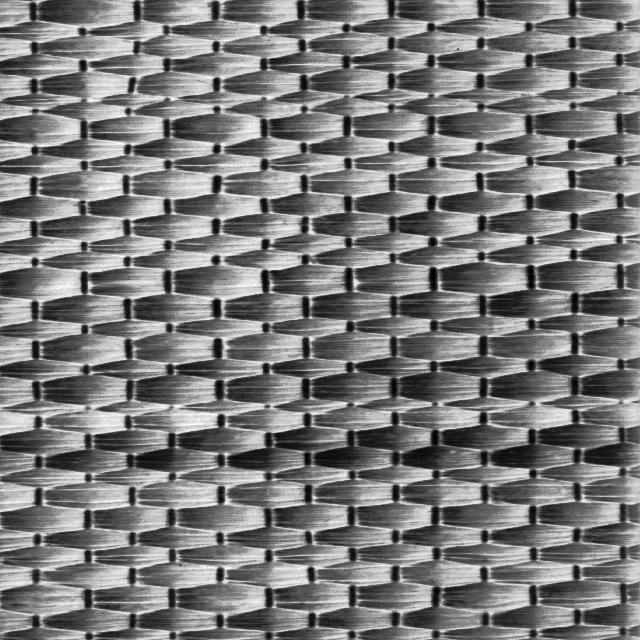
\includegraphics[width=\textwidth]{contenu/resources/images/lattice2}
    \end{subfigure}
    \hspace{1em}
    \begin{subfigure}[b]{.25\textwidth}
        \centering
        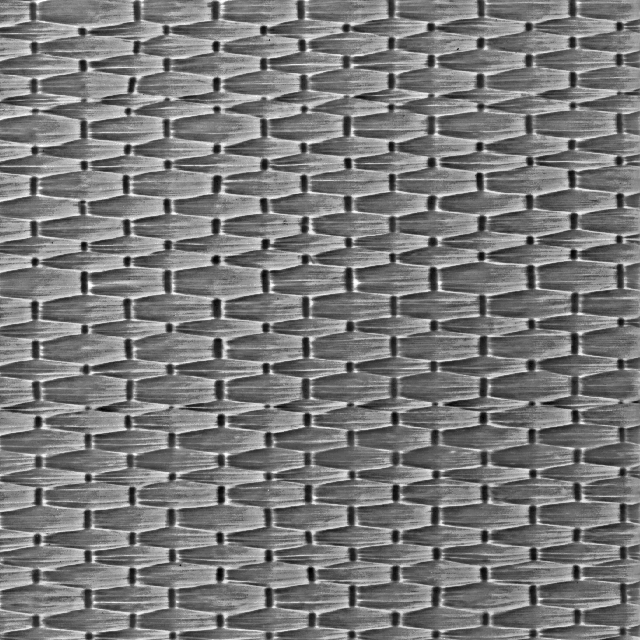
\includegraphics[width=\textwidth]{contenu/resources/images/lattice2_filtered}
    \end{subfigure}

    \caption[Filtrage de bandes de basses fréquences]{Filtrages de bandes de basses fréquences. Cette opération permet de supprimer les tâches présentes sur les textures, tout en conservant la structure globale et les détails. Les images originales (gauche) sont comparées aux images reconstruites sans certains niveaux de la pyramide (droite). Typiquement, seuls les deux premiers niveaux sont gardés, ainsi que le dernier, le résidu basse fréquence. Textures tirées de la base de textures Brodatz~\cite{abdelmounaime_new_2013}.}
    \label{fig:filter-low-freq}
\end{figure}

\section{Synthèse de texture préservant la congruence de phases}

L'intérêt principal et raison d'être du cadre de travail présenté précédemment est néanmoins l'utilisation de la congruence de phases, notamment en tant qu'indicatrice de la proximité à un bord. Cette mesure se comporte en effet comme un gradient dans la direction perpendiculaire au bord et permet de savoir ponctuellement si un texel se situe proche d'un bord. Avoir des informations de proximité à un bord par texel est particulièrement utile dans un contexte de calcul parallèle, comme celui du pipeline graphique. Un problème des calculs parallèles sur la carte graphique est en effet la perte d'information sur le contexte local. Avoir accès à la congruence de phases offre une solution à ce problème en donnant des informations sur le voisinage du fragment considéré.

\bigskip

Quelques expériences ont été faites pour exploiter le principe de voisinage, puis une méthode de synthèse de texture a été mise au point pour traiter les textures à structure irrégulière. Cette étude s'est intéressée à un type de textures en particulier, qui présentent des caractéristiques communes. Les textures considérées sont caractérisées par la présence de pavés de toute sorte, entre lesquels se trouve un matériau unique que nous appelons arrière-plan. Ces textures représentent souvent des sols. Quelques exemples sont montrés à la figure~\ref{fig:typical-textures}.

\bigskip

\begin{figure}
    \centering
    \begin{subfigure}{.3\textwidth}
        \centering
        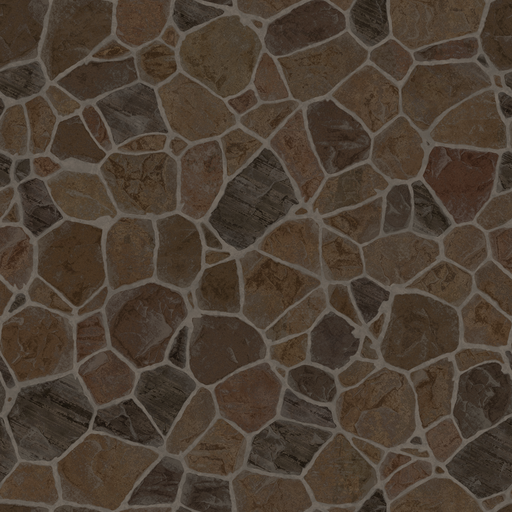
\includegraphics[width=\textwidth]{contenu/resources/images/texture_1}
    \end{subfigure}
    \hfill
    \begin{subfigure}{.3\textwidth}
        \centering
        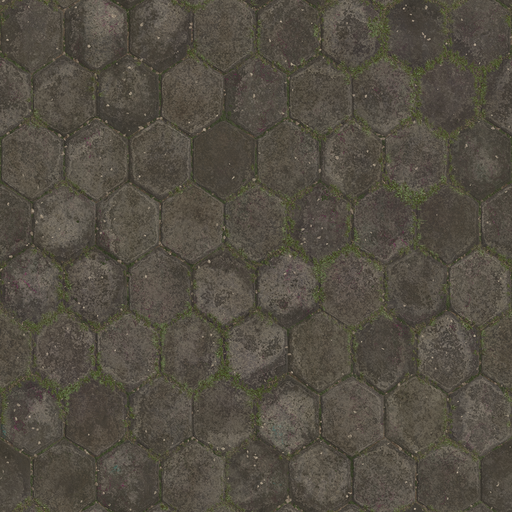
\includegraphics[width=\textwidth]{contenu/resources/images/texture_2}
    \end{subfigure}
    \hfill
    \begin{subfigure}{.3\textwidth}
        \centering
        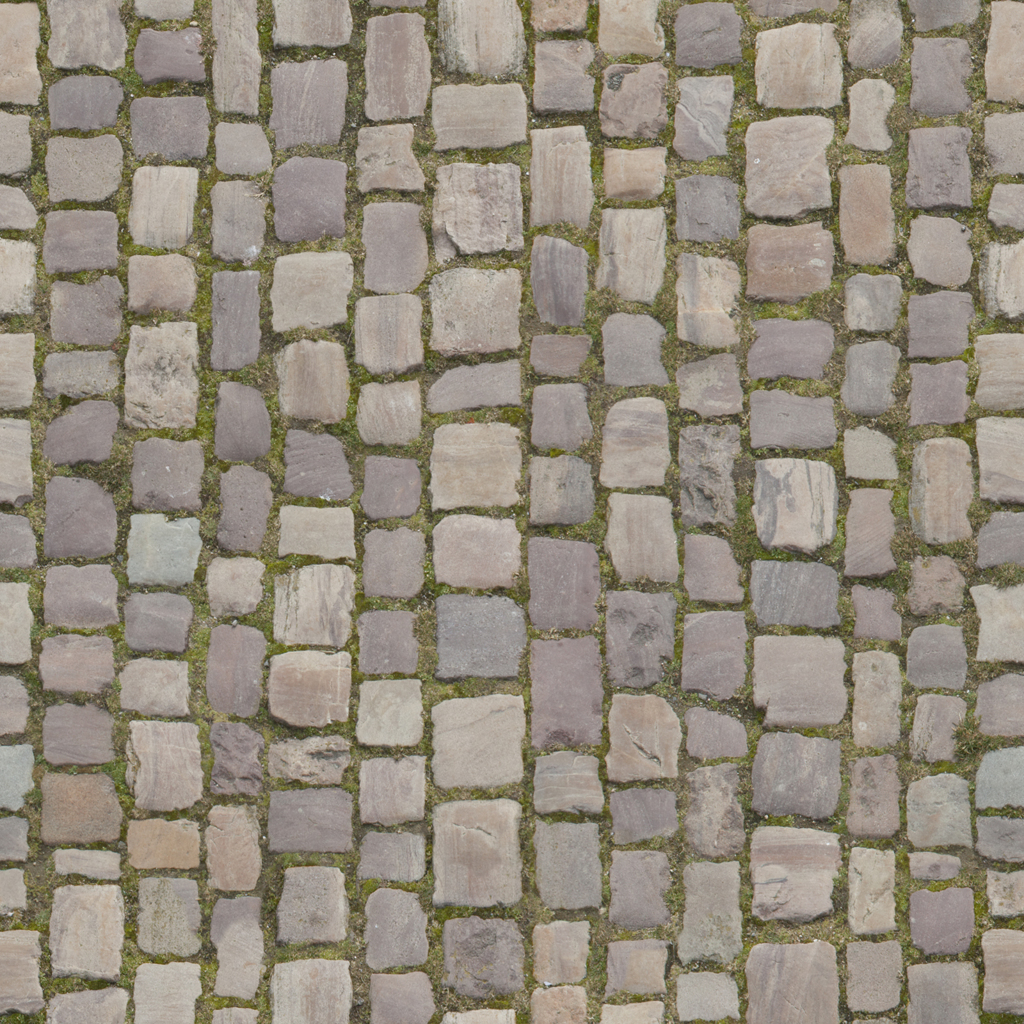
\includegraphics[width=\textwidth]{contenu/resources/images/texture_3}
    \end{subfigure}

    \caption{Exemples du genre de textures à structure irrégulière considérées.}
    \label{fig:typical-textures}
\end{figure}


Lutz \textit{et al.}~\cite{lutz_preserving_2023} font le constat que les méthodes de synthèse par pavage apériodique échouent à préserver la fonction d'autocovariance de l'exemple. Une synthèse par pavage apériodique est une sorte de synthèse par réorganisation reposant sur un échantillonnage uniforme de l'exemple d'entrée. Des corrélations qui contribuent à préserver l'apparence de l'entrée sont mal reproduites, ce qui donne un air trop aléatoire au résultat. Pour mieux préserver les corrélations de l'exemple, ils améliorent l'étape d'échantillonnage en utilisant le principe d'échantillonnage préférentiel. L'échantillonnage préférentiel consiste à influer l'échantillonnage en fonction d'une fonction de densité de probabilité. En utilisant la fonction d'autocovariance comme densité de probabilité, ils montrent que les corrélations sont mieux préservées et que la synthèse est de meilleure qualité car elle préserve mieux l'apparence.

\bigskip

Cette idée a été appliquée au cadre d'étude utilisé. Nous avons émis l'hypothèse que deux échantillons de contenu provenant d'une même composante, avec une congruence de phases similaire, ont un profil de couleurs similaire, puisqu'ils se situent à une même distance d'un bord. Pour vérifier cette hypothèse, une méthode de synthèse préservant la congruence de phases de l'exemple a été mise au point. Le principe de la synthèse proposée est de réorganiser le contenu de l'exemple à l'aide d'un échantillonneur préférentiel. L'échantillonneur utilisé indique, à chaque endroit, un contenu de remplacement possible. Pour chaque fragment de l'image à synthétiser, l'échantillonneur prend en compte la position du fragment dans la texture pour trouver un contenu de remplacement idéal et créer de la nouveauté. Différentes propriétés sont prises en considération pour calculer cette indirection. Les étapes de cette méthode sont détaillées dans la section qui suit.

\bigskip

Pour la mise au point de méthode de synthèse, nous avons décidé de travailler avec le contenu le plus petit possible pour la réorganisation : le pixel. Il y a des avantages à travailler avec des petites régions de pixels plutôt que des pixels unitaires et plusieurs méthodes de la littérature font ce choix~\cite{wei_state_2009}. Le choix de travailler avec des pixels a cependant été fait pour avoir un premier prototype rapide et pouvoir tester notre hypothèse. L'utilisation de l'échantillonneur s'adapte en effet particulièrement bien à l'échelle du pixel, contrairement à la synthèse par patch, qui demande plus d'efforts de mise en place.

\subsection{Échantillonneur préservant la congruence de phases}

Pour mettre en place l'échantillonneur, la stratégie proposée par Pharr \textit{et al.} dans leur livre~\cite{pharr_physically_2023} est reprise. L'échantillonnage de Pharr \textit{et al.} utilise la méthode de la transformée inverse. Cette méthode d'échantillonnage repose sur le fait que l'échantillonnage d'une variable aléatoire de loi donnée peut se faire par l'échantillonnage d'une variable aléatoire uniforme et l'application de la fonction de répartition inverse de la loi. L'avantage de la méthode de la transformée inverse est que l'échantillonnage d'une variable de loi uniforme est facile, contrairement à celui d'une variable de loi quelconque. Pour appliquer la méthode d'échantillonnage de Pharr \textit{et al.}, il faut dans un premier temps définir l'échantillonnage d'une fonction constante par morceaux 1D. Soit une fonction $f$ constante par morceaux
\begin{equation}
    f(x) = \left\{
        \begin{array}{ll}
            v_0 & \mbox{si } x \in [x_0, x_1] \\
            v_1 & \mbox{si } x \in [x_1, x_2] \\
            \vdots & \vdots \\
            v_{N-1} & \mbox{si } x \in [x_{N-1}, x_N]
        \end{array}
    \right.
\end{equation}
d'intégrale $I$
\begin{equation}
    I = \int_{0}^{1} f(x) dx = \sum_{i=0}^{N-1} \frac{v_i}N.
\end{equation}
Sans perte de généralité, $f$ est définie entre 0 et 1 et les $x_i$ sont disposés de manière régulière $x_i = i / N$. La fonction de densité de probabilité associée à $f$ est alors $p(x) = f(x) / I$. La fonction de répartition $F$ est linéaire par morceaux, définie aux $x_i$ et de coefficient directeur $v_i/I$ entre $x_i$ et $x_{i+1}$. Elle s'exprime par
\begin{equation}
    F(x_i) = \int_{0}^{x_i} p(t) dt = \sum_{j=0}^{x_i} \frac{v_j}{NI} = F(x_i-1) + \frac{v_i-1}{NI}.
\end{equation}
L'échantillonnage de $f$ se fait en échantillonnant une variable aléatoire uniforme $u$ et en calculant $F^{-1}(u)$.

\bigskip

% TODONT finish diagram perhaps, to show inversion method on 1D piecewise constant function
%\begin{tikzpicture}
%    \begin{axis}[
%        title={Fonction de répartition},
%        symbolic x coords={$x_0$, $x_1$, $x_2$, $x_3$},
%        ybar stacked,
%        ytick={0, 1}
%    ]
%        \addplot coordinates {
%            (x_0,0.3) (x_1,0.3) (x_2,0.3) (x_3,0.3)
%        };
%        \addplot coordinates {
%            (x_1, 0.2) (x_2, 0.2) (x_3, 0.2)
%        };
%        \addplot coordinates {
%            (x_2, 0.4) (x_3, 0.4)
%        };
%        \addplot coordinates {
%            (x_3, .1)
%        };
%
%        \node [above] at (0, 0.15) {$p_1$};
%        \node [above] at (1, 0.15) {$p_1$};
%        \node [above] at (0, 0.15) {$p_1$};
%        \node [above] at (0, 0.15) {$p_1$};
%
%    \end{axis}
%
%\end{tikzpicture}

Il faut ensuite constater que les textures sont des tableaux, donc des fonctions constantes par morceaux 2D. Les lois de probabilité conditionnelle et marginale sont des fonctions constantes par morceaux 1D. La stratégie est ainsi d'échantillonner la probabilité marginale pour avoir la première coordonnée, puis d'échantillonner la probabilité conditionnelle en utilisant la première valeur trouvée pour déterminer la seconde coordonnée.

\subsection{Synthèse avec l'échantillonneur préférentiel}

Le principe d'échantillonnage préférentiel est utilisé pour synthétiser du nouveau contenu, en préservant la fonction de congruence de phases. La synthèse se fait en tirant, pour chaque fragment, un nouveau contenu avec une valeur de congruence de phases similaire. L'idéal serait d'avoir une fonction de densité de probabilité adaptée pour chaque valeur. La fonction de densité idéale privilégierait l'échantillonnage des valeurs autour de $x$ pour tout $x$ dans l'espace des valeurs possibles. Il est cependant compliqué de stocker une fonction de densité pour une mesure à valeurs continues. Pour résoudre le problème, une quantification en $N$ intervalles de taille constante $1/N$ est réalisée. L'intervalle $i$ ne contient que les valeurs entre $[i/N, (i+1)/N[$. Ce sont les intervalles quantifiés qui servent de densité de probabilité pour l'échantillonnage préférentiel. En pratique, la quantification se fait avec $N=10$ intervalles et le partitionnement est fait entre les valeurs minimum et maximum calculées, plutôt qu'entre 0 et 1 (qui sont les extremums théoriques). Au moment de tirer du nouveau contenu, la valeur de congruence de phases du fragment à remplacer est évaluée en échantillonnant une carte stockée en mémoire. Un contenu de remplacement est trouvé en utilisant l'échantillonneur avec l'intervalle de congruence de phases correspondant à la valeur échantillonnée.

\bigskip

Pour préserver la cohérence dans l'image, les contenus provenant de différentes composantes de la texture ne doivent pas être mélangés. Les textures étudiées ont souvent deux composantes, les pavés et l'arrière-plan. L'image est donc partitionnée entre les différentes composantes à l'aide d'une classification par l'algorithme des K-moyennes. Pour chaque composante, un masque binaire est créé et appliqué sur les intervalles de congruence de phases par multiplication, pour obtenir la densité de probabilité finale pour chaque composante et chaque niveau de congruence.

\bigskip

Pour utiliser efficacement l'échantillonneur dans la synthèse en temps-réel, une première étape de pré-calcul hors-ligne est nécessaire. Plusieurs réalisations de l'échantillonneur sont calculées, pour chaque composante et pour chaque intervalle de congruence de phases, afin d'augmenter la variété de l'échantillonneur. Les réalisations de l'échantillonneur sont des vecteurs de translations $(u, v)$ stockés dans une carte de texture pour être chargés sur la carte graphique. La texture stockant les réalisations de l'échantillonneur est un jeu de données à trois dimensions : une pour les subdivisions de la congruence de phases, une pour les différentes composantes et la dernière pour les différentes réalisations de l'échantillonneur. Un schéma explicatif est montré à la figure~\ref{fig:sampler-realization}.

\bigskip

\begin{figure}
    \centering
    \begin{subfigure}{.5\textwidth}
        \centering
        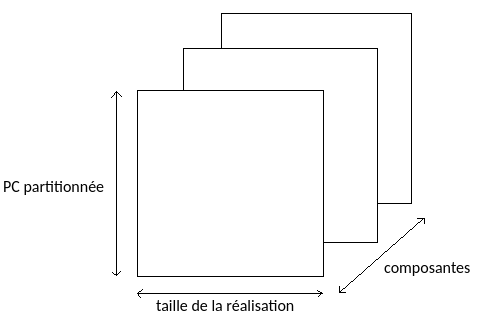
\includegraphics[width=\textwidth]{contenu/resources/images/sampler_realization}
    \end{subfigure}
    \hfill
    \begin{subfigure}{.45\textwidth}
        \centering
        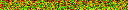
\includegraphics[width=\textwidth]{contenu/resources/images/realization_pc_0}
    \end{subfigure}

    \caption[Réalisation de l'échantillonneur préférentiel]{Schéma explicatif de la texture 3D où la réalisation de l'échantillonneur est stockée (gauche) et un exemple de réalisation pour une composante avec 10 niveaux de subdivisions de congruence de phases et 128 échantillons (droite).}
    \label{fig:sampler-realization}
\end{figure}

La texture de réalisation est ensuite utilisée dans le \textit{fragment shader} lors du rendu pour faire l'échantillonnage en temps-réel. La valeur de congruence de phases et la composante du fragment à remplacer sont échantillonnés, puis utilisés pour aller chercher la bonne réalisation dans la texture 3D. La réalisation est ensuite choisie aléatoirement entre toutes les réalisations qui ont la même congruence de phases et la même composante. En pratique, le choix de la réalisation se fait à l'aide d'une fonction de hachage, avec les coordonnées $(u, v)$ du fragment pour lequel l'échantillonnage est fait.

\bigskip

\begin{figure}
    \centering
    \begin{subfigure}{.95\textwidth}
        \centering
        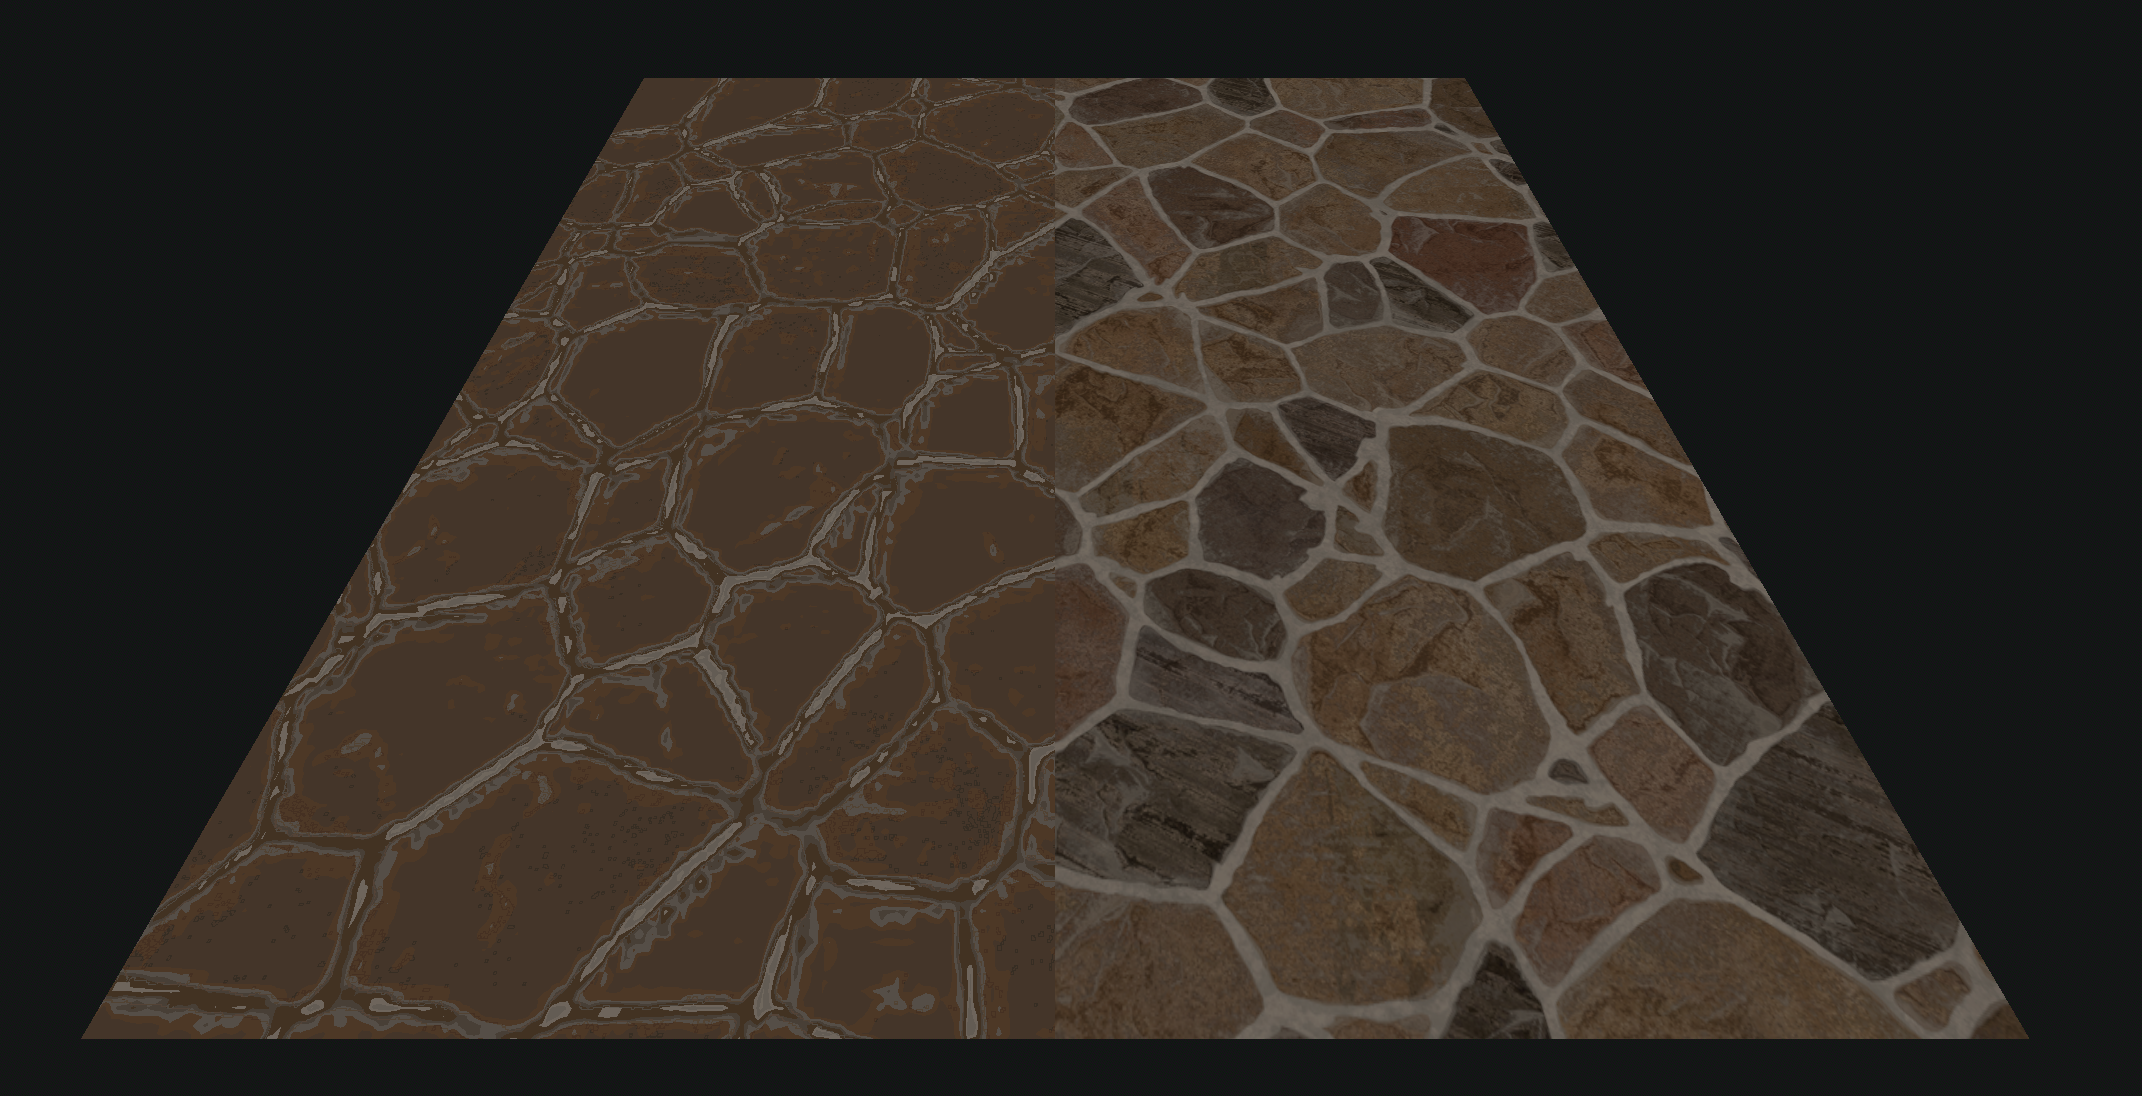
\includegraphics[width=\textwidth]{contenu/resources/images/partitioned_sampling_pc_preserving_no_shuffle}
    \end{subfigure}
    \\
    \begin{subfigure}{.95\textwidth}
        \centering
        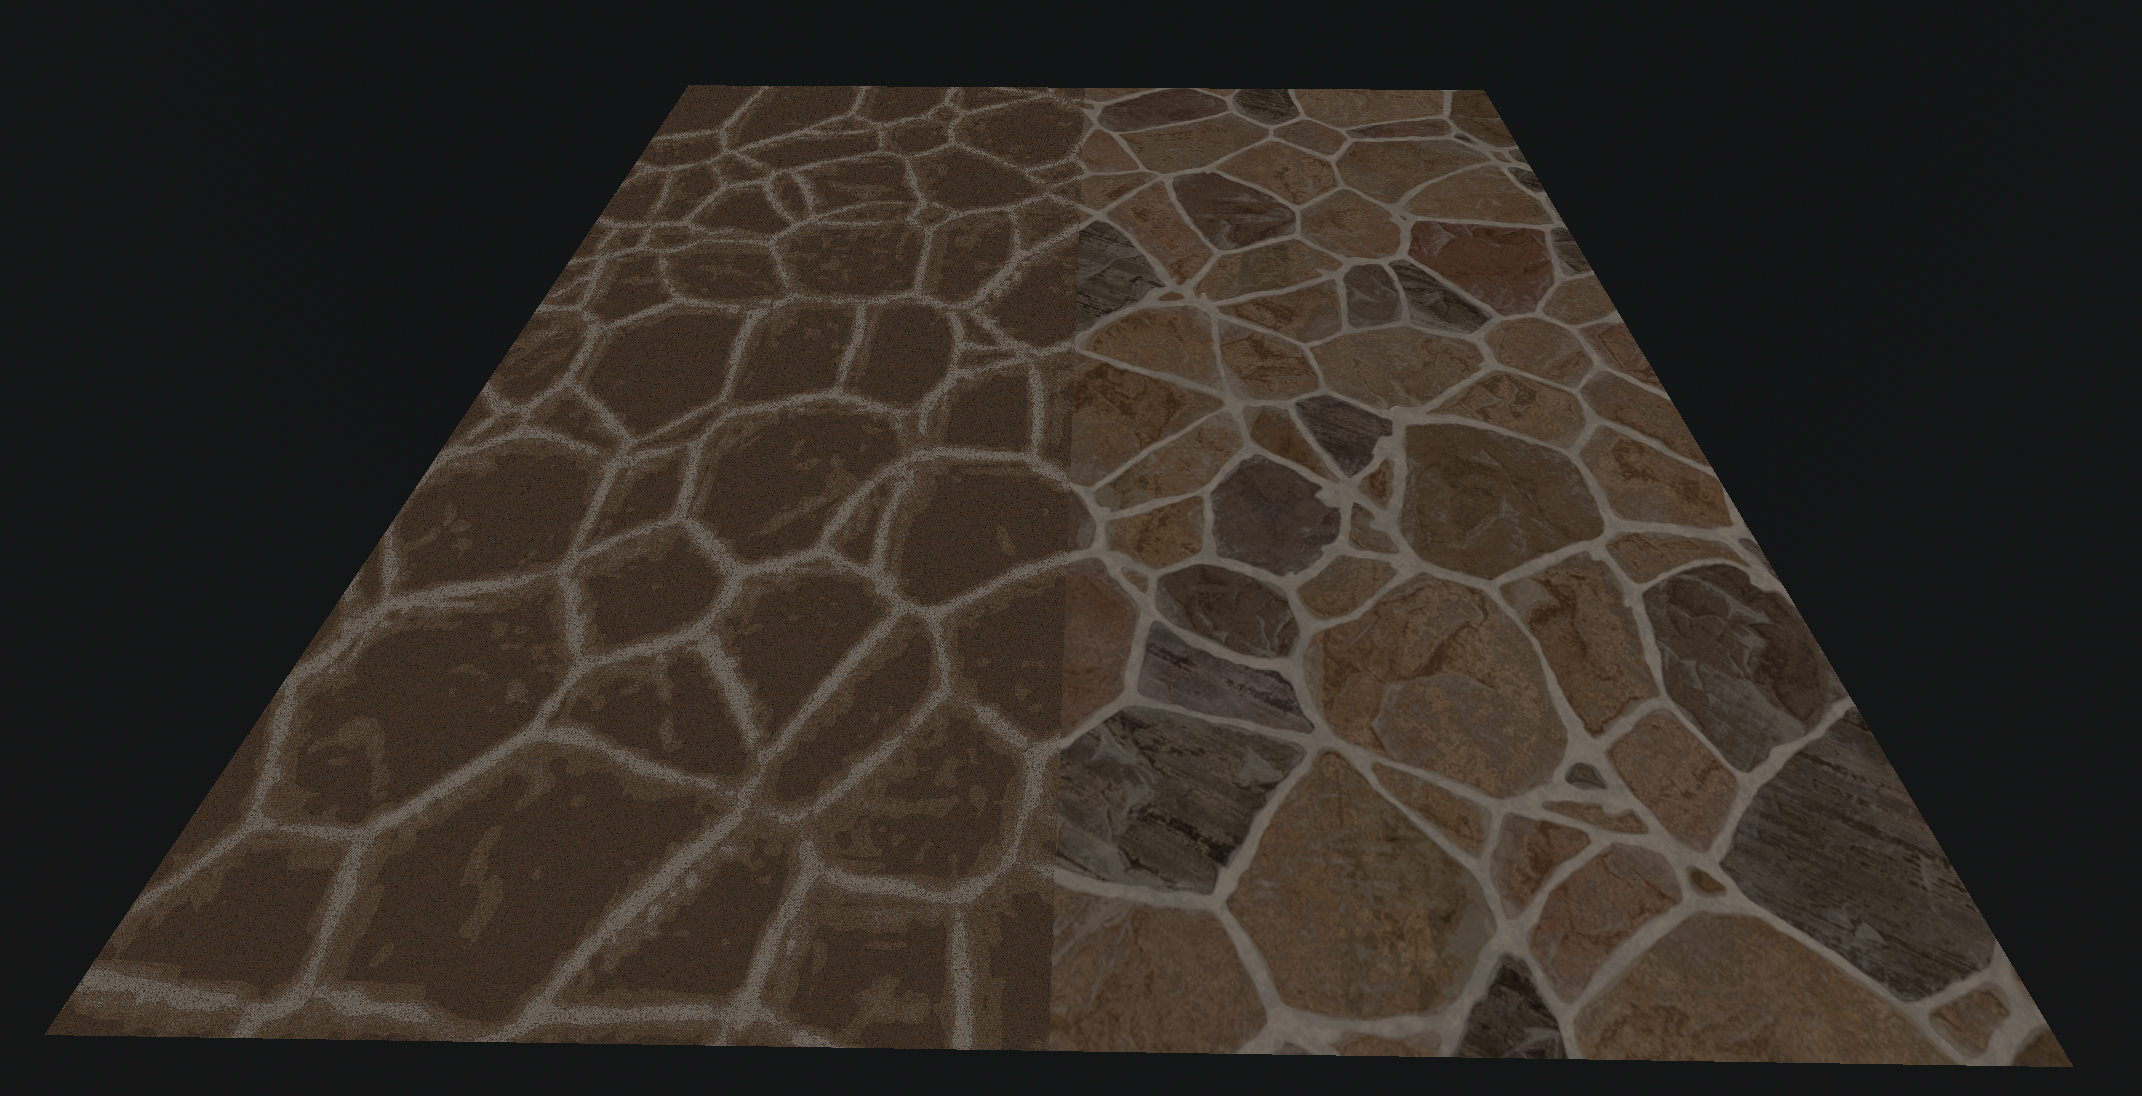
\includegraphics[width=\textwidth]{contenu/resources/images/partitioned_sampling_pc_preserving_shuffle_uv}
    \end{subfigure}
    \caption[Échantillonnage avec et sans multiples réalisations]{Comparaison du résultat de l'échantillonnage avec et sans multiples réalisations. La partie de droite de chaque image montre la texture originale. L'échantillonnage avec une seule réalisation (haut) donne le même échantillonnage pour plusieurs pixels alors qu'utiliser plusieurs réalisations (bas) apporte de la variété.}
    \label{fig:offset-shuffle}
\end{figure}

Pour savoir quel pixel remplacer lors de l'évaluation du \textit{fragment shader}, le pavage périodique est utilisé. L'exemple d'entrée est dupliqué et déplacé pour couvrir la surface à remplir. Les coordonnées de texture du fragment sont utilisées pour savoir quel pixel de l'exemple d'entrée aller chercher. Il est ainsi possible de calculer la congruence de phases de l'exemple d'entrée et de l'utiliser pour échantillonner le nouveau contenu. Le pavage périodique est connu pour créer des artefacts visuels, notamment des motifs de répétition. Cependant, nous pensons que l'utilisation de l'échantillonneur pourra atténuer ces artefacts en apportant de la variété dans l'échantillonnage.

\begin{figure}[t]
    \centering
    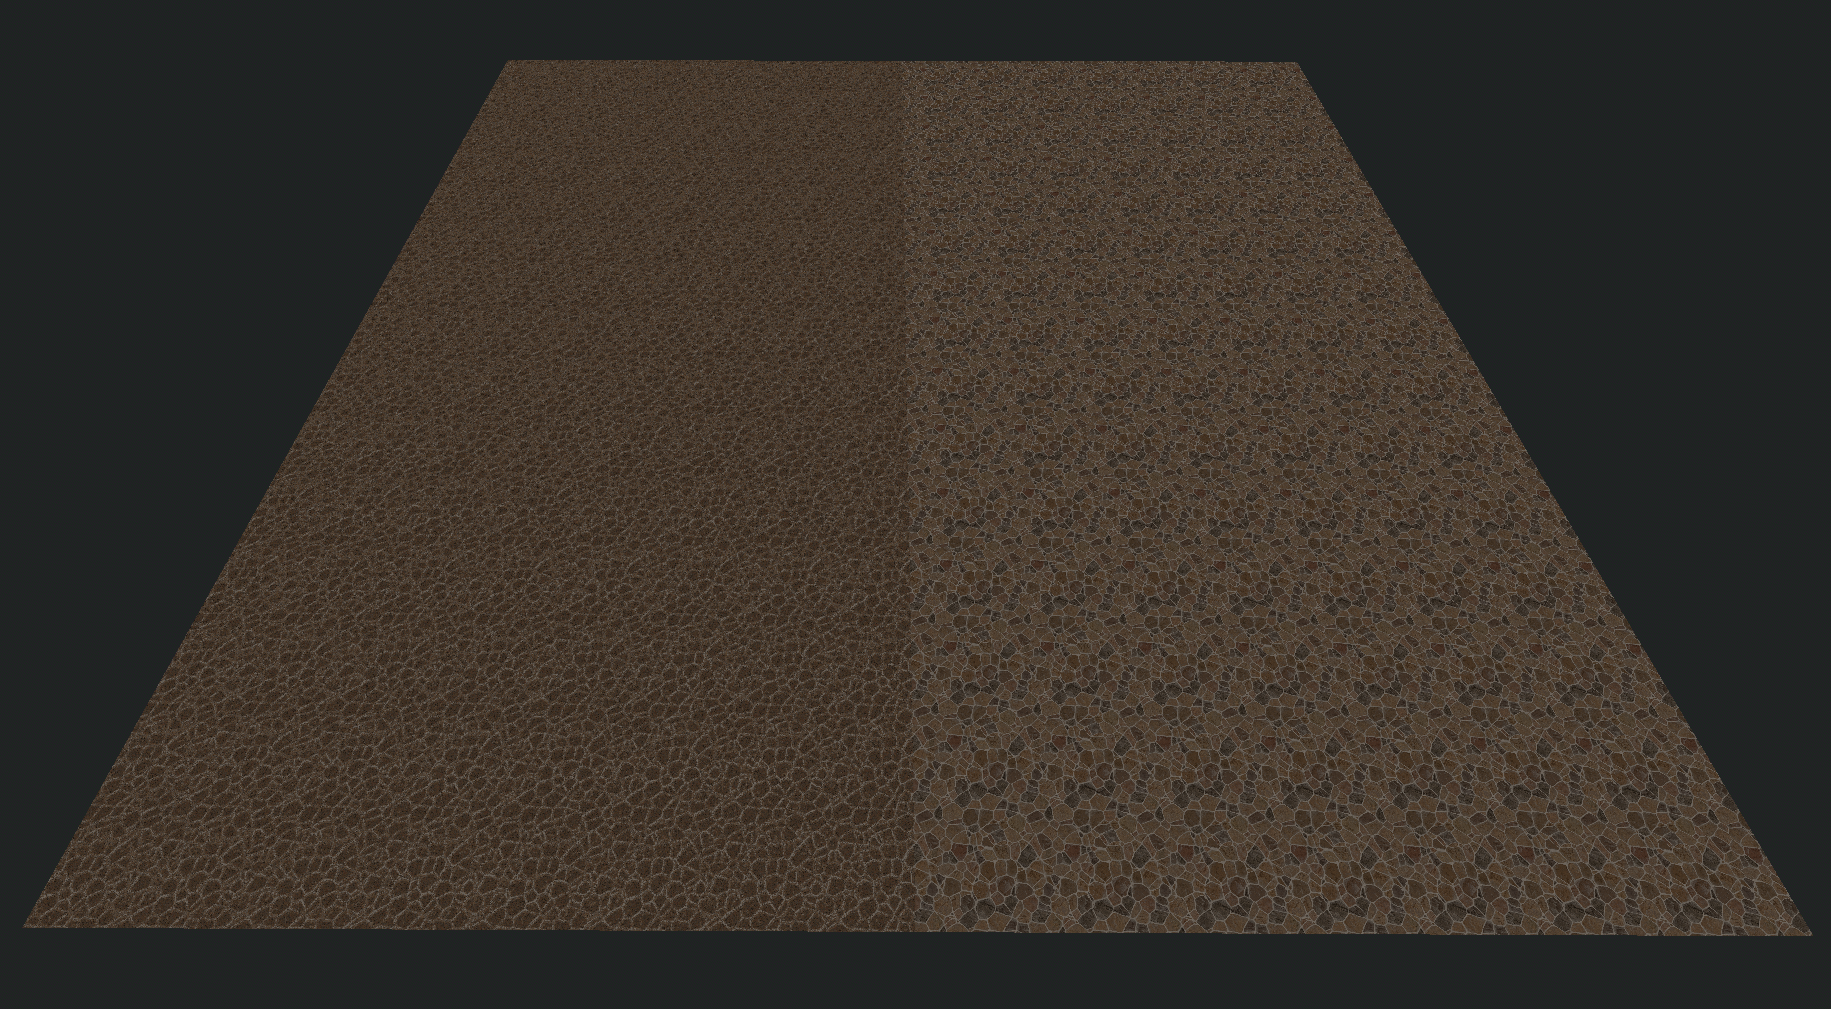
\includegraphics[width=\textwidth]{contenu/resources/images/partitioned_sampling_pc_preserving_shuffle_uv_far}
    \caption[Résultat de l'échantillonnage avec multiples réalisations, vu de loin]{Résultat de l'échantillonnage avec multiples réalisations, vu de loin. L'échantillonnage préférentiel permet d'atténuer les artefacts visuels dûs à la répétition du pavage périodique. La partie droite de la surface est recouverte par un pavage périodique classique.}
    \label{fig:pc-preserving-synthesis}
\end{figure}

\section{Discussion}

Dans ce chapitre, plusieurs applications de la congruence de phases ont été présentées, à savoir la sélection de niveaux de fréquences et la synthèse de texture préservant la structure. Une analyse des résultats obtenus est faite et une discussion sur les limites et implications de l'approche proposée est présentée.

\paragraph{Sélection de niveaux de fréquences}

La sélection de niveaux de fréquences par l'élimination de niveaux de la pyramide d'image est une méthode qui permet de visualiser différentes échelles de structure présentes dans l'image. Les différents niveaux de structure distingués dans une image sont liés à certaines fréquences dans le domaine spectral et donc à différents niveaux de la pyramide d'image. Étudier et sélectionner différents niveaux de la pyramide permet de mieux comprendre la structure de l'image. La sélection de niveaux de fréquences a été mise à profit pour faire du filtrage de bandes de basses fréquences pour effacer des tâches présentes sur des textures, comme présenté en figure~\ref{fig:filter-low-freq}. Une méthode similaire a d'ailleurs été publiée~\cite{zhang_pyramid_2023} indépendamment du travail décrit dans ce manuscrit, au cours des derniers mois de la recherche. Les deux méthodes n'ont pas été comparées, car ce n'était pas le but de cette recherche.

\bigskip

Le processus présente cependant des désavantages. D'abord, il relève d'un travail manuel. L'utilisateur doit lui-même observer les congruences de phases partielles, qui ne comportent pas tous les étages de la pyramide, et décider lesquelles supprimer ou garder. La tâche peut être fastidieuse et manque de métrique de décision pour automatiser et homogénéiser la démarche. De plus, la méthode souffre du problème que les bandes de fréquences parasites sont parfois corrélées à du contenu qu'il serait souhaitable de préserver. Il est alors impossible avec cette méthode d'ôter précisément le contenu indésirable, sans affecter le reste de la texture.

\paragraph{Synthèse de texture préservant la congruence de phases}
\label{par:discussion-synthesis}

La synthèse de texture préservant la congruence de phases est la deuxième application et est au cœur de ce travail. La synthèse proposée est un prototype de recherche mis au point pour examiner notre hypothèse : la congruence de phases, qui est un indicateur de la proximité d'un bord, donne aussi une mesure de ressemblance entre plusieurs contenus d'une texture. La synthèse de texture préservant la congruence de phases ne permet pas la synthèse de texture utilisable dans un environnement virtuel telle quelle, mais a mené à plusieurs observations sur l'utilisation de la congruence de phases appliquée au domaine de la synthèse de texture.

\bigskip

Les résultats montrés en figure~\ref{fig:pc-preserving-synthesis} indiquent que la congruence de phases seule ne suffit pas à capturer la similarité entre deux contenus. Sur la figure, la couleur des pavés reconstruits tend vers un marron uniforme. Les pavés de la texture originale ont des couleurs variées, mais la synthèse donne une couleur uniforme, la même pour tous les pavés. La méthode d'échantillonnage ne prend pas en compte la couleur de chaque pavé et échantillonne sans distinction dans des pavés de couleurs différentes. Même si la congruence de phases est préservée, la couleur est mélangée et la variété diminue.

\bigskip

La congruence de phases semble cependant bien détecter et, dans une certaine mesure préserver, des éléments de structure internes aux pavés. À la figure~\ref{fig:mark-preserved} que les marques ou fissures dans les pavés sont encore présentes après la synthèse. Cette caractéristique a néanmoins un désavantage : l'échantillonneur ne fait pas de distinction entre le bord d'un pavé et le bord d'une marque à l'intérieur d'un pavé, comme montré à la figure~\ref{fig:pc-defect}. Des pixels sont échantillonnés au mauvais endroit et le contenu des bords et des marques des pavés sont mélangés, ce qui n'est pas désirable.

\bigskip

\begin{figure}
    \centering
    \begin{subfigure}{.45\textwidth}
        \centering
        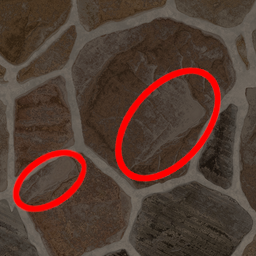
\includegraphics[width=\textwidth]{contenu/resources/images/marks}
    \end{subfigure}
    \hfill
    \begin{subfigure}{.45\textwidth}
        \centering
        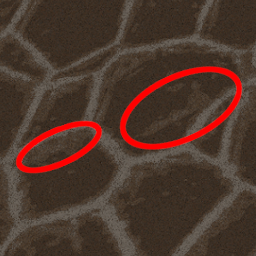
\includegraphics[width=\textwidth]{contenu/resources/images/mark_preserved}
    \end{subfigure}

    \caption[L'échantillonneur préserve partiellement les marques dans les pavés]{Zoom sur deux marques présentes au sein d'un pavé de la texture (gauche) qui se retrouvent sur la texture synthétisée avec l'échantillonneur préservant la congruence de phases (droite).}
    \label{fig:mark-preserved}
\end{figure}

\begin{figure}
    \centering
    \begin{subfigure}{.45\textwidth}
        \centering
        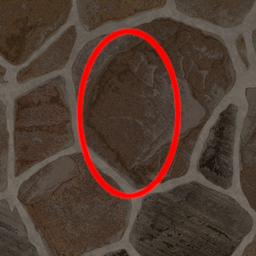
\includegraphics[width=\textwidth]{contenu/resources/images/stone_zoom}
    \end{subfigure}
    \hfill
    \begin{subfigure}{.45\textwidth}
        \centering
        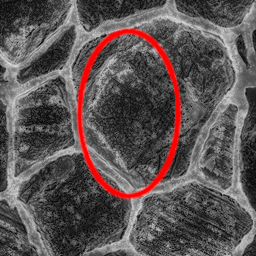
\includegraphics[width=\textwidth]{contenu/resources/images/stone_zoom_pc}
    \end{subfigure}

    \caption[Problème d'échantillonnage dû à la présence de marques au sein des pavés de la texture]{Zoom sur une marque présente au sein d'un pavé de la texture (gauche) et la congruence de phases associée à cette zone (droite). La congruence de phases a des valeurs semblables sur les bords du pavé et autour de la marque foncée mise en évidence. Cela cause des problème pour l'échantillonnage.}
    \label{fig:pc-defect}
\end{figure}

Le mélange des couleurs observé est aussi dû au choix de travailler avec des pixels unitaires plutôt que des petites régions de pixels. En agissant au niveau du pixel, la préservation de la congruence de phases à elle seule n'est pas suffisante pour préserver des corrélations locales comme la couleur. Il faudrait travailler avec des régions de pixels pour avoir du contenu moins décorrélé de son entourage ou trouver une manière d'accorder une plus grande importance au voisinage local lors de l'échantillonnage du nouveau contenu.

\bigskip

Enfin une dernière observation est que la synthèse gagnerait en variété si une disposition des pixels autre qu'un pavage périodique était utilisée. Le choix du pavage périodique est une question de simplicité, car le sujet de l'étude est l'échantillonneur plutôt que la disposition. L'utilisation de l'échantillonneur permet d'atténuer les artefacts visuels dûs à la répétition du pavage périodique. Cependant les artefacts visuels sont encore visibles lorsque la texture est observée de loin, comme à la figure~\ref{fig:pc-preserving-synthesis}. La recherche de méthode d'organisation de contenu pour générer des nouvelles dispositions (par exemple des pavés de forme similaire, mais différente à tous les autres pavés de l'exemple) en temps réel est néanmoins un sujet difficile et reste encore ouvert aujourd'hui~\cite{baldi_differentiable_2023, guehl_semi-procedural_2020}.
